\section{Methodology}

\subsection{Data Preprocessing}
\label{subsec:Data_Preprocessing}

\subsubsection{Sample blacklist}

As already mentioned in \fullref{subsec:Data_exploration_and_visualization}, a significant amount of pictures in the dataset are likely to negatively impact the learning of the mode. Our flower recognition model is intended to be used in an application where the images are supposed be focused on one or few flowers of the same type, from a close to middle-range distance (1 to 10 meters), in natural colours.

The black-listing of pictures aim to discard samples:
\begin{itemize}
	\setlength\itemsep{1pt}
	\setlength{\parskip}{0pt}
	\setlength{\parsep}{0pt}
	\item which don't have a ".jpg" extension (some python web scrapping routine can be found in the \textit{dandelion} subfolder)
	\item not representing a flower
	\item wrongly classified
	\item containing other subjects (persons, insects, objects,...)
	\item close ups
	\item wide shots with fields, mountains, landscapes...
	\item drawings
	\item with artistic filters significantly denaturing the original colour
\end{itemize}

After the manual visualization of all samples, the blacklist contains 1059 items (24.5\% of the total dataset) stored in a text file (\texttt{blacklist.txt}). The data loading implementation read this file and discards any file found in the list. 

\begin{center}
	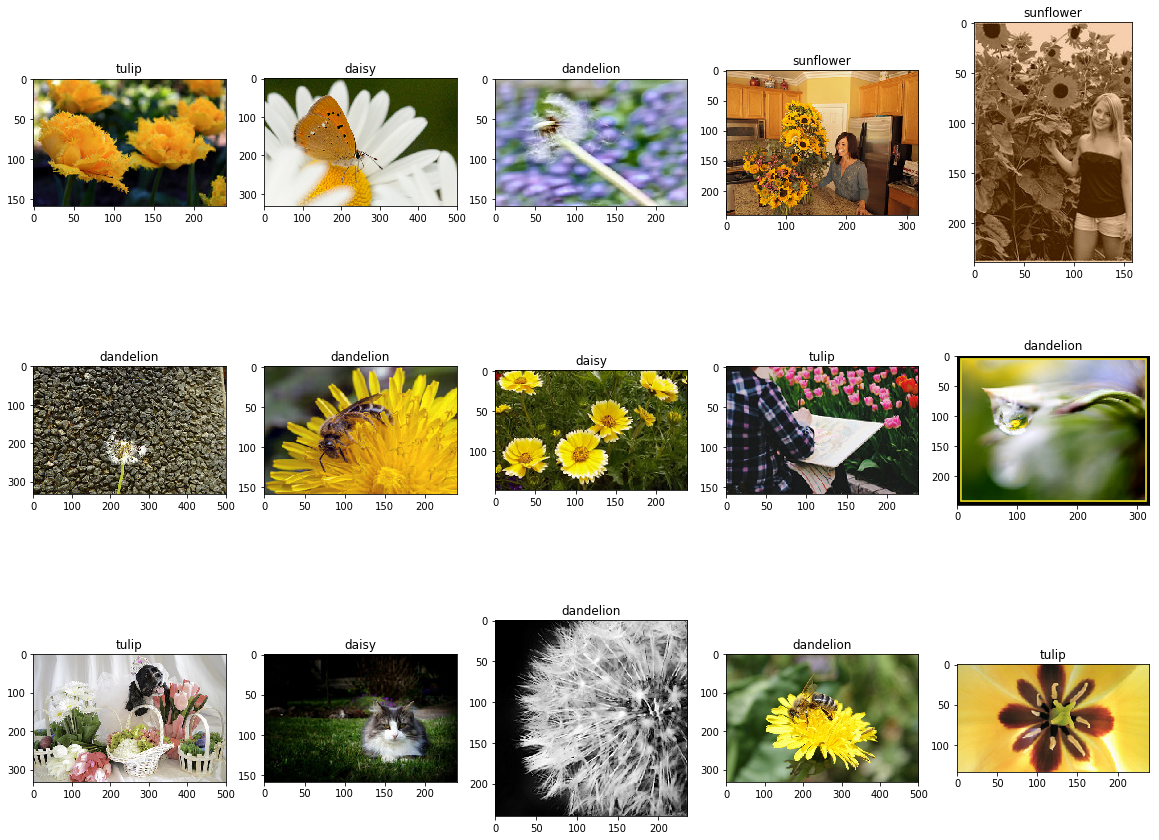
\includegraphics[scale=.35]{./sections/03_methodology/output_11_1.png}
	\captionof{figure}{samples of black listed pictures}
\end{center}

%\captionof{program}{picture file scan and filtering}
%\begin{python}
%from sklearn.datasets import load_files 
%	
%path = "./flowers"
%
%blacklist_file = "blacklist.txt" # list of files to be removed drm the dataset
%
%#read blacklist
%with open(blacklist_file, 'r') as f:
%	blacklist = f.readlines()
%blacklist = [path + s.strip() for s in blacklist]
%
%# scan all files stored in the data folder
%data = load_files(path, load_content=False)
%all_flowers_files = np.array([s.replace('\\', '/') for s in data["filenames"]])
%
%# identify blacklist indexes
%isvalid_file = [True if f not in blacklist else False for f in all_flowers_files]
%flowers_files = all_flowers_files[isvalid_file]
%
%# flowers_targets = np_utils.to_categorical(data["target"],5)
%flowers_targets = data["target"][isvalid_file]
%flowers_target_names = data["target_names"]
%\end{python}

After filtering, we observe that the  new classes distribution is comparable to the original one. The classes are ow represented by 654 samples on average:

\begin{flushleft}
	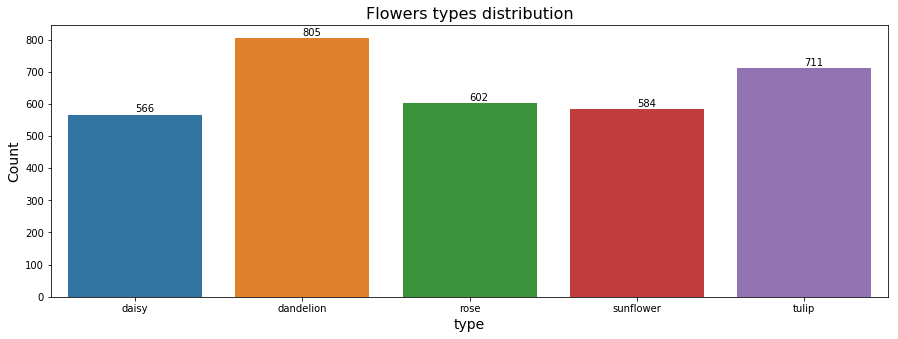
\includegraphics[scale=.5]{./sections/03_methodology/output_13_0.png}
	\captionof{figure}{Images distribution after blacklist filtering}
\end{flushleft}

\subsubsection{Training, validation and testing split}

The dataset is randomly split in 3 parts using the \texttt{train\_test\_split} from \texttt{sklearn.model\_selection} package, using the \texttt{stratify} option in order to preserve the original classes distribution in each split:

\begin{itemize}
	\setlength\itemsep{1pt}
	\setlength{\parskip}{0pt}
	\setlength{\parsep}{0pt}
	\item Training (76.5\% - 2500 samples)
	\item Validation (8.5\% - 278 samples)
	\item Testing (15\% - 491 samples)
\end{itemize}

%\captionof{program}{picture files train/valid/test split}
%\begin{python}
%from sklearn.model_selection import train_test_split	
%	
%# train+valid / test split
%test_size = .1
%
%flowers_files_train_valid, flowers_files_test, flowers_targets_train_valid, flowers_targets_test = train_test_split(
%flowers_files, flowers_targets, 
%test_size = test_size, 
%stratify=flowers_targets)
%
%# train / valid split
%valid_size = .2
%flowers_files_train, flowers_files_valid, flowers_targets_train, flowers_targets_valid = train_test_split(
%flowers_files_train_valid, flowers_targets_train_valid, 
%test_size = valid_size, 
%stratify=flowers_targets_train_valid)
%\end{python}

\begin{flushleft}
	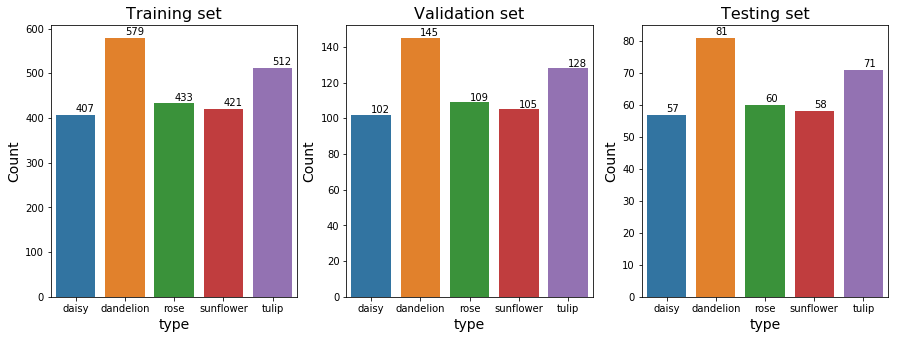
\includegraphics[scale=.5]{./sections/03_methodology/output_18_0.png}
	\captionof{figure}{Stratified images distributions after train/valid/test split}
\end{flushleft}

\subsubsection{Dataset loading in memory}

The images are loaded in RBG colors and resized in a 299x299 shape using OpenCV "\texttt{cv2}" python package. 
Targets labels are one-hot-encoded using the \texttt{to\_categorical} method from the \texttt{keras.utils.np\_utils} package.

%\captionof{program}{Image loading with openCV}
%\begin{python}
%from keras.utils import np_utils
%from tqdm import tqdm
%import cv2
%
%def loadimg(path):
%	"""
%	load and resize an image
%	return a (299, 299, 3) array
%	"""
%	img = cv2.imread(path)
%	img_r = cv2.resize(img, (299, 299))
%	return img_r
%
%x_train = np.array([loadimg(f) for f in tqdm(flowers_files_train)]).reshape(-1, 299, 299, 3)
%y_train =  np_utils.to_categorical(flowers_targets_train)
%
%x_valid = np.array([loadimg(f) for f in tqdm(flowers_files_valid)]).reshape(-1, 299, 299, 3)
%y_valid =  np_utils.to_categorical(flowers_targets_valid)
%
%x_test = np.array([loadimg(f) for f in tqdm(flowers_files_test)]).reshape(-1, 299, 299, 3)
%y_test =  np_utils.to_categorical(flowers_targets_test)
%
%\end{python}

\subsubsection{Image augmentation}
\label{subsubsec:Image_augmentation}

In order to enrich the dataset, image augmentation is applied to the training and validation datasets using the \texttt{ImageDataGenerator} utility from the \texttt{keras.preprocessing.image} package. This step is also used to normalize the features: all values are divided by 255. 
No image augmentation is applied on the testing set which is meant to represent real case images for the model evaluation. 

%\captionof{program}{Augmented image generators}
%\begin{python}
%	from keras.preprocessing.image import ImageDataGenerator
%	train_datagen = ImageDataGenerator(
%	rescale=1./255,
%	shear_range=0.2,
%	zoom_range=0.2,
%	horizontal_flip=True)
%\end{python}

\begin{center}
	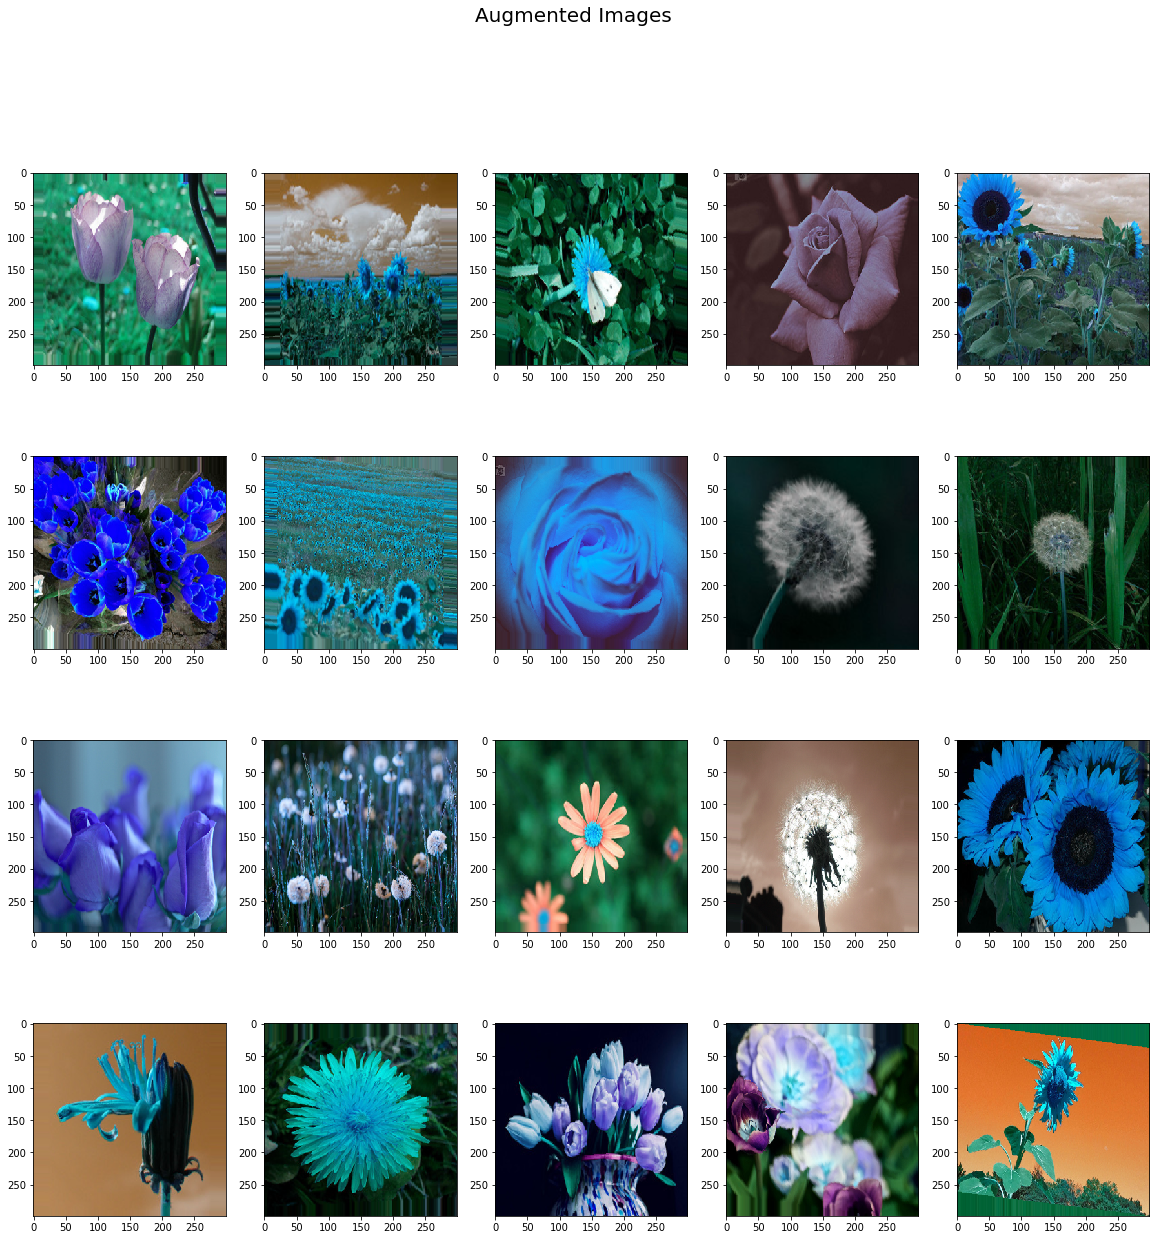
\includegraphics[scale=.3]{./sections/03_methodology/output_26_0.png}
	\captionof{figure}{samples of augmented training images}
\end{center}

\subsection{Model Implementation}

\subsubsection{CNN architecture}

The targeted CNN architecture is the combination of a fixed weights base model and some custom top layers specialized for the prediction of flower varieties. Hyper-parameters such as learning and decay rates have been determined experimentally and tested in order to find th best learning time/accuracy compromise. 
\\

\underline{\textbf{Model design:}}

The overall model design procedure consists of the following steps:

\begin{enumerate}
	\setlength\itemsep{1pt}
	\setlength{\parskip}{0pt}
	\setlength{\parsep}{0pt}
	\item load the weights of a base model trained on ImageNet dataset, without the top layers, setting the input shape to (299,299,3).
	\item freeze the base model weights
	\item Add top layers 
	\item compile the model with loss function, optimizer and metrics set-up
\end{enumerate}

\underline{\textbf{Top layers:}}

The top layers consist of the following:

\begin{itemize}
	\setlength\itemsep{1pt}
	\setlength{\parskip}{0pt}
	\setlength{\parsep}{0pt}
	\item a flatten layer connected to the last convolution layer of the base model (usually a MaxPooling layer)
	\item a fully connected layer with ReLu activation. A number of 500 units has been arbitrarily chosen. 
	\item a dropout layer. A dropout factor of 0.3 has been determined experimentally. 
	\item an output layer with 5 units (1 for each flower class) and a \textit{softmax} activation function. 
\end{itemize}

\underline{\textbf{Hyper-parameters:}}

\begin{itemize}
	\setlength\itemsep{1pt}
	\setlength{\parskip}{0pt}
	\setlength{\parsep}{0pt}
	\item Optimizer: Adam with learning rate $\alpha=1e^-3$ and decay $d=1e^-6$ 
	\item loss function: categorical cross-entropy
	\item metrics : accuracy
\end{itemize}

This architecture is inspired by the solution proposed by A. Akashnian in his "Flowers are mesmerizing" notebook published on \href{https://www.kaggle.com/aakashnain/flowers-are-mesmerizing}{Kaggle.com}  \cite{NAIN_notebook}.

%\captionof{program}{construction of a CNN with VGG16 as base model}
%\begin{python}
%from keras.applications.vgg16 import VGG16
%from keras.layers import Flatten, Dense, Dropout
%from keras.models import Model
%from keras.optimizers import Adam
%
%# load the base model, do not include top layers
%base_model = VGG16(weights='imagenet', include_top=False, input_shape=(299,299,3))  
%
%# freeze the layers of the base model
%for layer in base_model.layers:
%	layer.trainable = False   
%
%# top layers:
%x = Flatten()(base_model.output)
%x = Dense(500, activation='relu', name='fc1')(x)
%x = Dropout(0.3)(x)
%x = Dense(5, activation='softmax', name='fc2')(x)
%
%model = Model(inputs=base_model.input, outputs=x)
%
%# set up the optimizer
%opt = Adam(lr = 1e-3, decay=1e-6)
%
%# compile the model
%model.compile(loss = 'categorical_crossentropy', optimizer=opt, metrics=['accuracy'])
%\end{python}

\subsubsection{CNN training}

The model is trained with the augmented pictures generator specified in \fullref{subsubsec:Image_augmentation},  on 50 epochs with batches of 32 samples (= 73 steps/epoch). The model weights are saved via a \texttt{ModelCheckpoint} each time that the validation loss each a new minima. The training historic is stored in order to later analyse the accuracies and losses evolution during the training. In order to speed-up the processing time, the model has been trained on an Amazon Web Services GPU instance (50 to 60 seconds per epochs).

%\captionof{program}{model training}
%\begin{python}
%from keras.callbacks import ModelCheckpoint 
%	
%batch_size = 32
%epochs = 50
%saved_models_dir = 'saved_models'
%
%#if it doesn't exist, create the saved model directory 
%if not os.path.isdir(saved_models_dir):
%	os.mkdir(saved_models_dir)
%
%# define the model weight h5 storage
%best_weights_h5 = os.path.join(saved_models_dir,
%	'weights.best.flowers_recognition.{}.hdf5'.format(base_model_name))
%
%# model checkpointer
%checkpointer = ModelCheckpoint(filepath=best_weights_h5, 
%	verbose=1, save_best_only=True)
%
%# training
%training_hist = model.fit_generator(train_datagen.flow(x_train, y_train, batch_size=batch_size),
%	steps_per_epoch=x_train.shape[0] // batch_size,
%	epochs=epochs, 
%	verbose=1, 
%	callbacks=[checkpointer],
%	validation_data=valid_datagen.flow(x_valid, y_valid, batch_size=batch_size),
%	validation_steps=x_valid.shape[0] // batch_size)
%	
%\end{python}

\subsection{Model Refinement}

\subsubsection{Base Model selection}

The \texttt{keras.applications} package offers some pre-trained models. In frame of this project, the \texttt{VGG16}, \texttt{VGG19} and \texttt{Resnet50} based models have been individually tested on 10 epochs. 

%--- VGG16 based model
\begin{center}
	\centering
	\begin{minipage}{0.5\textwidth}
		\centering
		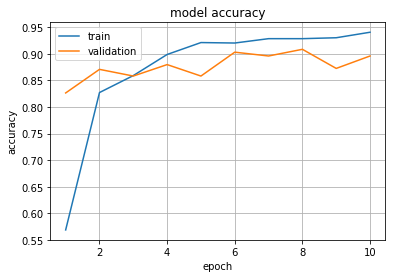
\includegraphics[width=0.9\textwidth]{./sections/03_methodology/VGG16_10epochs_acc.png}
		\captionof{figure}{VGG16 - 10 epochs Accuracy}
		\label{VGG16_10e_Acc}
	\end{minipage}\hfill
	\begin{minipage}{0.5\textwidth}
		\centering
		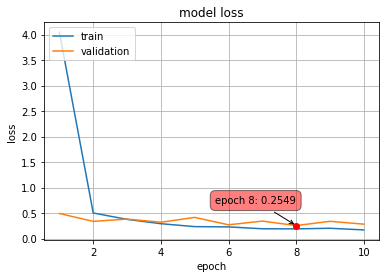
\includegraphics[width=0.9\textwidth]{./sections/03_methodology/VGG16_10epochs_loss.png} 
		\captionof{figure}{VGG16 - 10 epochs Loss}
		\label{VGG16_10e_Loss}
	\end{minipage}
\end{center}

According to Fig. \ref{VGG16_10e_Acc} and \ref{VGG16_10e_Loss}, VGG16 based model seems to learn extremely fast after the first back-propagation at epoch 1. It then constantly improves during the next epochs. After 10 epochs, the best validation loss achieved is 0.2549  and the accuracy 0.91 at epoch 8. This base model seems to be a good candidate for our flowers classifier.

--- VGG19
\begin{center}
	\centering
	\begin{minipage}{0.5\textwidth}
		\centering
		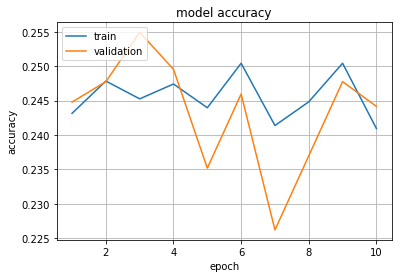
\includegraphics[width=0.9\textwidth]{./sections/03_methodology/VGG19_10epochs_acc.png}
		\captionof{figure}{VGG19 - 10 epochs Accuracy}
		\label{VGG19_10e_Acc}
	\end{minipage}\hfill
	\begin{minipage}{0.5\textwidth}
		\centering
		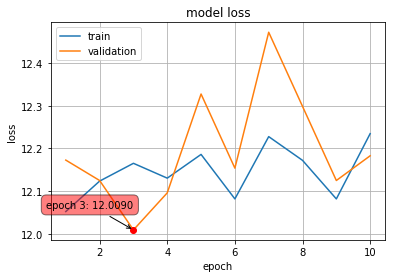
\includegraphics[width=0.9\textwidth]{./sections/03_methodology/VGG19_10epochs_loss.png} 
		\captionof{figure}{VGG19 - 10 epochs Loss}
		\label{VGG19_10e_Loss}
	\end{minipage}
\end{center}

According to Fig. \ref{VGG19_10e_Acc} and \ref{VGG19_10e_Loss}, the VGG19 based model doesn't seem able to learn. The average training accuracy of 24\% is comparable to random guesses performance. This base model will not be considered for the flower classifier.

%---Resnet50
\begin{center}
	\centering
	\begin{minipage}{0.5\textwidth}
		\centering
		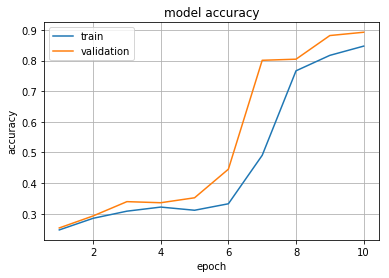
\includegraphics[width=0.9\textwidth]{./sections/03_methodology/Resnet50_10epochs_acc.png}
		\captionof{figure}{Resnet50 - 10 epochs Accuracy}
		\label{resnet50_10e_Acc}
	\end{minipage}\hfill
	\begin{minipage}{0.5\textwidth}
		\centering
		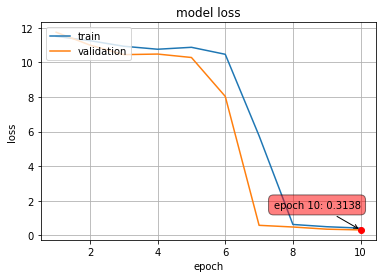
\includegraphics[width=0.9\textwidth]{./sections/03_methodology/Resnet50_10epochs_loss.png} 
		\captionof{figure}{Resnet50 - 10 epochs Loss}
		\label{resnet50_10e_Loss}
	\end{minipage}
\end{center}

According to Fig. \ref{resnet50_10e_Acc} and \ref{resnet50_10e_Loss}, it takes up to 7 epochs for this model to achieve reasonably good performances. It reach its best validation loss at the 10th epoch with 0.3138 and an accuracy of nearly 90\%, letting suggest that it could even more improve with longer training. 
\\\\
\textbf{\underline{base model selection - conclusion:}}

The best performing flower classifier on 10 epochs is the \textbf{VGG16 based model}. Therefore, it has been selected to perform a full training on 50 epochs.
